\documentclass{article}

\usepackage[letterpaper]{geometry}
\geometry{top=.5in, bottom=1.0in, left=1.0in, right=1.0in}
\usepackage{url}
\usepackage{hyperref}
\usepackage{float}
\usepackage{graphicx}
\usepackage{amsmath}
\usepackage{moreverb} % for verbatimtab 
\usepackage{framed}

\usepackage{verbatim}

\newenvironment{code}{\framed  \verbatimtab  }{ \noindent \\[-1cm]\endverbatimtab \endframed }


\title{
Memory Management Review} \author{Todd, gauglertodd@gmail.com}
\begin{document}
\maketitle
\noindent \\[-1cm]

\tableofcontents

\section{Physical Address Space? Logical Address Space? Wat?}
Here's the definition from Wikipedia: \emph{In computing, a Physical address (also real address, or binary address), is a memory address that is represented in the form of a binary number on the address bus circuitry in order to enable the data bus to access a particular storage cell of main memory, or a register of memory mapped I/O device.} The physical address is the address loaded into the memory address register of the actual memory, the physical address (or `absolute address') is an actual location in the main memory. 

\begin{figure}[h]
\centering
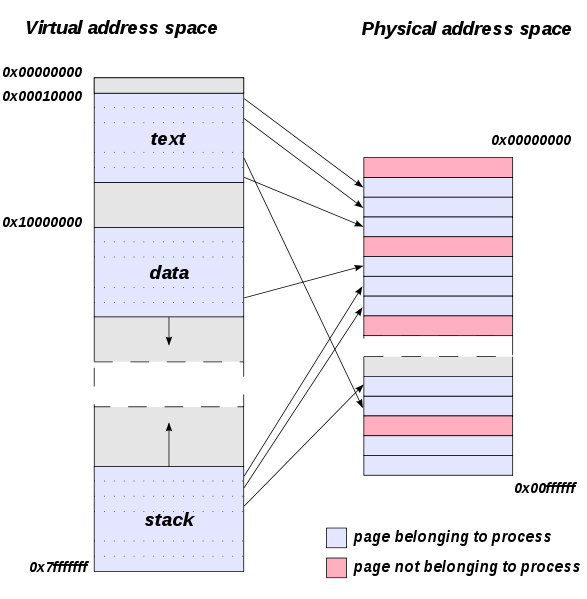
\includegraphics[scale=.7]{fig1.png}
\end{figure}


Alternatively, the logical address is the address `generated by the CPU', where the physical address is the \emph{actual address of the process in memory}. The CPU generates the logical address that is added with an offset value to get the actual address of a process in the memory. 

The logical address space is really just the set of all logical addresses generated by some program (and similarly, the physical address space is the set of all physical addresses). 

From the interweb, 

\emph{
Logical address is the address generated by the CPU (from the perspective of a program that is running) whereas physical address (or the real address) is the address seen by the memory unit and it allows the data bus to access a particular memory cell in the main memory. All the logical addresses need to be mapped in to physical addresses before they can be used by the MMU. Physical and logical addresses are same when using compile time and load time address binding but they differ when using execution time address binding.
}
\url{http://www.differencebetween.com/difference-between-logical-address-and-vs-physical-address/}

\section{Contiguous Allocation}


The main memory must accommodate both the operating system and the various user processes. We therefore need to allocate different parts of the main memory in the most efficient way possible.

The memory is usually divided into two partitions: one for the resident operating system, and one for the user processes. We may place the operating system in either low memeory or high memory. With this approach each process is contained in a single contiguous section of memory.

One of the simplest methods for memory allocation is to divide memory into several fixed-sized partitions. Each partition may contain exactly one process. In this multiple-partition method, when a partition is free, a process is selected from the input queue and is loaded into the free partition. When the process terminates, the partition becomes available for another process. The operating system keeps a table indicating which parts of memory are available and which are occupied. Finally, when a process arrives and needs memory, a memory section large enough for this process is provided.

Note: Depending on the method used, this approach can suffer from external as well as internal memory fragmentation.

\url{http://www.cs.iit.edu/~cs561/cs351/memory_management_FS_sched/index_mm_03.html}


In single partition allocation there is a single user space memory partition protected with relocation and limit registers. Processes are swapped in and out to provide for multiprogramming.
You want to protect the operating-system code and data from changes by user processes and also need to protect user processes from one another, and you can do this with a relocation register (it contains the value of the smallest physical address) and the limit register (which contains the range of logical addresses). It should look something like this:
\begin{figure}[h]
\centering
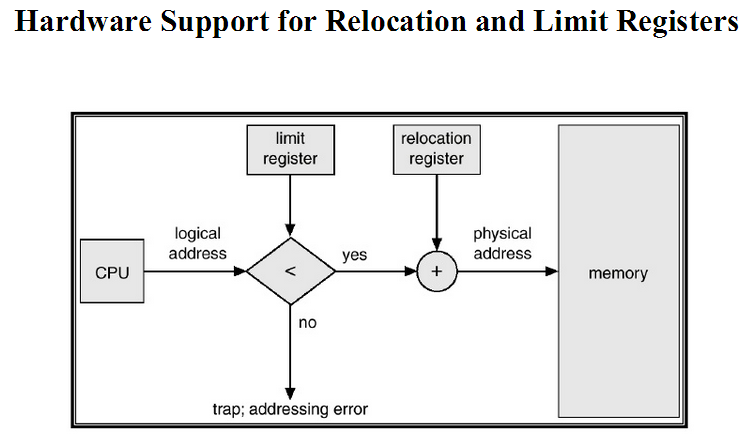
\includegraphics[scale=.7]{fig2.png}
\end{figure}

The MMU (memory-management unit) is a device that maps virtual to physical addresses, and it does so by adding the value in the relocation register to every address generated by a uswer process. \url{http://www.cs.odu.edu/~cs471w/spring12/lectures/MainMemory.htm}




\begin{figure}[h]
\centering
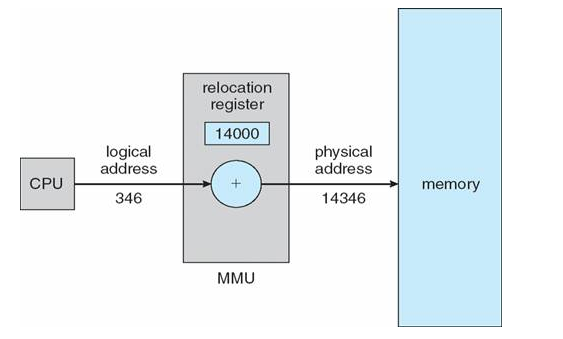
\includegraphics[scale=.7]{fig3.png}
\end{figure}


We have to now consider { \bf Multiple Partition Contiguous Memory Allocation}: a problem arises, you need to allocate available memory to various processes that are in the job queue waiting to be brought into memory. There's a cool presentation on this idea here: \url{http://cs.uttyler.edu/Faculty/Rainwater/COSC3355/Animations/multiplepartcma.htm}. 

You can partition the main memory in two obvious ways, you can partition it into equal sized chunks, or into unequal sized chunks. They both have their advantages and disadvantages: fixed sized partitions make it entirely inconsequential as to which partition you put a job into (so placement algorithms are really simple), but one problem is that the number of partitions is predefined and limits the total number of active
processes in the system. Additionally, partition sizes are preset and small jobs don't run efficiently, as they're given waaay more space than they need. You can sort of handle this issue with unequal sized partitions, but then you have to increase the complexity of your placement algorithms, and some queues might be empty while some might be loaded, which is a bad thing for some reason.




\url{https://docs.google.com/viewer?a=v&q=cache:1qwkgN29YgAJ:u.cs.biu.ac.il/~ariel/download/os288/ppts/os7-2_rea.ppt+&hl=en&gl=us&pid=bl&srcid=ADGEESjnCEowgcJ8051GQ_YDdwRD0H8qMtEihlmdxf-9FdAW7CuC9kn4TWKu71y7rt14Lv8FnL06W0eGA2X2rqjNNX_5J9bEbjWCD6tBbjfla93POJdEytYpJAg_Wq1JkxFi6rIRPIkp&sig=AHIEtbSFeOd4XJguMsogSrjRgysNF_BQFw}





The best thing to do is to start using {\bf Dynamic Partitioning}. The idea here is that the partitions used are of a variable length (and there are a variable amount of them). When a process is brought into main memory, it is given \emph{exactly} as much memory as it needs. The OS keeps a table to track the parts of memory that are open/occupied, and initially the memory is considered as one great big single block of available memory (called a \emph{hole}). As processes enter the system, they get put into a queue, and at any given time there is a list of available block sizes that the input queue can interact with. The OS can order the input queue according to a scheduling algorithm, when a process arrives and needs some amount of memory, it simply searches for a large enough memory hole. If a hole is too big it gets split in two, one part is given to the process and the other is given to the set of available holes. When a process terminates, it releases the block of memory it was using (see another cool presentation here \url{http://www.cs.jhu.edu/~yairamir/cs418/os5/sld014.htm}). This leads to the fairly natural question of, `oh crap, I need to fit something into memory, it's of size $n$, where the heck do I put it?'. Here are some of the common strategies used:
\begin{enumerate}
\item {\bf First Fit}: just allocate the first big enough hole that you can find. Searching can start at the beginning of your set of holes, or where the previous first-fit search ended. 
\item {\bf Best Fit}: allocate the smallest hole that can provide memory for your process.
\item {\bf Worst-Fit}: allocate the largest possible hole. This then gives you the largest leftover hole after you split the largest hole into two separate partitions. 
\end{enumerate}

This then leads us to have to deal with {\bf external fragmentation}, which is when you actually have enough total memory space to satisfy the request of a process, but the memory is broken up (isn't contiguous), so you can't actually put the process anywhere in a convenient manner. The solution to this problem is {\bf compaction}, where you shuffle all the free space around so that all the free memory is together in one large contiguous block. This process of compaction is only possible if the reallocation of memory is dynamic and done at execution time. The issues with it are that coming up with a optimal compaction strategy is kind of pain in the butt. Alternatively, you can combine swapping with compaction. 

Her notes on internal fragmentation are crap, so I pulled this definition off wikipedia: \emph{Due to the rules governing memory allocation, more computer memory is sometimes allocated than is needed. For example, memory can only be provided to programs in chunks divisible by 4, 8 or 16, and as a result if a program requests perhaps 23 bytes, it will actually get a chunk of 24. When this happens, the excess memory goes to waste. In this scenario, the unusable memory is contained within an allocated region, and is thus termed {\bf internal fragmentation}}


\url{http://en.wikipedia.org/wiki/Fragmentation_(computing)}.


\section{Paging}

As just discussed, external fragmentation causes problems because you can't really allocate memory in a nice way. There are non-nice ways to allocate this memory though; you can simply permit the logical addresses for a process to be non-contiguous via something called {\bf paging schemes}. In this idea, physical memory is broken into fixed-sized blocks of things called \emph{frames}, and the logical memory is broken into blocks of the same sized called \emph{pages} (Fluture's notes tell us that this size is `usually between 2 and 8K'. I have almost no idea what a 'K' is. ). There is this part of the hard disk that is used specifically by paging and swapping systems called the 'Backing Store', which is divided into fixed-sized blocks that are the same size as the memory frames. The page (whose size is supposed to be the same as the frame size) size is defined by the hardware, which depends on the computer architecture. 
(see \url{http://cs.uttyler.edu/Faculty/Rainwater/COSC3355/Animations/pagingmodel.htm} for a nice demonstration of this discussion). 

So here's the idea: your {\bf Page Table} is a mapping that assigns to each virtual page (logical memory) a page frame number, or auxiliary storage number. The page table the ncontains the base address of each page in physical memory. The {\bf Frame Table} contains information about the physical memory, how many total frames there are, which frames are allocated to which page of which process, and which frames are still available. 

Here is a summary of the process: if a process arrives to be executed, its size in pages is examined. Each page of the process needs a frame; if the process needs $n$ pages then there have to be at least $n$ frames available in memory. The first page of the process is loaded into one of the allocated frames, and the frame number is entered into the page table for this process. The second is loaded in the same way, and you do this until the process has the memory it needs. Here is a excerpt from the notes that tells us how to calculate the logical address: 

\begin{align*}
&\text{Logical Address:} &\text{ page number } (p) | & \text{ page offset }(d)\\
&&m-n   & \quad  n
\end{align*}
Where $p$ is an index into the page table, and $d$ is the displacement within the page. 

We also have the following formula: 
\begin{enumerate}
\item $S$ is the page size in bytes,
\item $R$ is the logical reference, and
\item $F$ is the frame number
\end{enumerate}
Then,
\[
\text{Physical Address} = f\cdot S + offset = f\cdot S +( R\mod S)
\]
There's even this way to calculate the address translation that uses Hardware support, and Fluture supplied the following formula in her notes:
\[
\text{physical address : frame number(f) | frame offset (displacement) d }
\]
which as a math major makes me want to kill someone. I don't have the first clue as to what this means.

The OS maintains a copy of the page table of each process, and this copy is used by the OS to map addresses. This page table is a set of {\bf dedicated registers}, and the `use of the registers for the page table is satisfactory if the page table is reasonable small'. Since this doesn't really mean anything to me in the English language, I ran to (you guessed it) the internet, and found the following \url{http://www.slideshare.net/guestff64339/implementation-of-page-table}. 

Reasonable questions about the page table include, `how do we implement it in hardware?', `how do we deal with with page sizes', and `what the heck was Fluture talking about when she wrote her notes on page tables?'. 

The page table is kept in main memory, and a {\bf page table base register} is a register that points to the page table. This is nice, because now changing page tables only makes you change this one register, which reduces context switch time. The table uses a fast-lookup hardware cache, called {\bf associative registers} or {\bf translation look-aside buffers (TLB's)}. The associative registers are only there to deal with a few of the page-table entries, if the page number is found in the associative registers then its number if immediately available. If not, then a memory reference to the page table must be made. This is fast, but the hardware itself is expensive. The {\bf hit ratio} is the percentage of times that a page number is found in the associative registers. 

\subsection{Address Translation with Hardware Support} 
There are three cases to consider here. 

\begin{enumerate}
\item Direct Mapping: In this situation, the page table is in primary memory, two memory accesses are needed to have access to a bite, and {\bf slowdown} happens when the page table has to be accessed in memory (it wasn't found simply in the associative registers). \url{http://nob.cs.ucdavis.edu/classes/ecs150-2008-02/handouts/memory/mm-pagat.html}.A given Main Memory block can be mapped to one and only one Cache Memory line.
It is Simple, Inexpensive, fast, but it lacks mapping flexibility. 

\item Associative Mapping: each register has a key and a value that is really the frame number. Every entry in the associative storage is searched simultaneously, which costs more in time as much more time is needed to search the associative registers. That being said, only a single memory reference is made. 

\item Combined Associative/Direct mapping: if the frame number is in the associative mapping, the searching process stops. Otherwise, search further on in the page table. In addition, the page number and frame number are added to the associative registers, so they will be found quickly upon future reference. 

The idea is to combine both mappings together to implement either a pure direct mapping or an associate register to implement a mapping. It's a nice compromise. 
\end{enumerate}

If $h=$TLB hit ratio, then
\begin{equation}
\text{ effective access time} = h\cdot \text{TLB hit access time} + (1-h)\cdot \text{TLB miss access time}
\end{equation}
where I assume that the hit/miss access times can be supplied. 

\section{Protection}
Memory protection in a paged environment is done through the use of protection bits that are associated with each frame. A bit can, for example, define a page to be read-write or read-only or execute-only: a {\bf valid-invalid} bit acts in a way that if the bit is set of `valid' then the reference is legal, and if the bit is set to `invalid' then the page is not in the process's logical address space.  What does this sentence mean exactly? See \url{http://www.scribd.com/doc/71013535/48/Valid-Invalid-Bit}, the idea is that a bit is associated to a page table where that bit's value is 1 if the process is in that memory, 0 otherwise. 

Sometimes in multiprogrammed computer systems, users want to run the same program twice. If you keep allocating space for each new program, then things can get out of hand. Instead, non-modifiable code is named `reentrant code' ,and is shared. If the code is reentrant, then it never changes throughout the execution of the processes. Certain heavily used programs can be shared, like database systems and compilers. However, modifiable code can't be shared - so we need the ability to identify each page as either sharable or nonsharable. 

So, we're going to have to talk about {\bf segmentation} \url{http://en.wikipedia.org/wiki/Memory_segmentation}. Suppose you'd rather deal with memory as these variable sized and unordered segments. Then, segmentation is the memory machagement schedme where a program occupies lots of seperate segments of memory, and they don't need to be the same size, or have to be adjacent to one another. The logical address will just be a collection of segments, which can represent procedures functions or data structures. Each segment gets a length and a name. Elements in a segment gets identified by their offset from the beginning of the segment; 
\[
\text{ logical address } \quad \langle \text{ segment number, offset }\rangle
\]

The mappings from user-defined addresses into these physical addresses is done by using a segment table, which can be implemented in fast registers or memory. Each table has variable length, and each entry of the table has a segment $base$ and a segment $limit$. When a process is running, a register (called the segment table base register) holds the starting address of the segment table for that process. BEcause the number of segments that a program uses varies, a segment table length register is also used (a STLR). 



























































\section{Some worked out questions}
Professor Fluture posted some questions that are apparently well-known, and not necessarily her own. This is actually really nice, because they are written well and have solutions from other people online. I found some examples, see below for the questions and links to answers. 



\begin{code}
9.8	Consider a logical-address space of eight pages of 1,024 words each, 
mapped onto a physical memory of 32 frames.
a.	How many bits are in the logical-address?	
b.	How many bits are in the physical address?

9.10	Consider a paging system with the page table stored in memory.
a.	If a memory reference takes 200 nanoseconds, how long does a paged memory 
reference take?
b.	If we add TLBs, and 75 percent of all page-table references are found in the
TLBs, what is the effective memory reference time? (Assume that finding a 
page-table entry in  the TLBs takes zero time, if the entry is there.)
\end{code}

\url{http://inst.eecs.berkeley.edu/~cs162/sp03/hw/hw3-solutions.html}

and 

\url{http://www.ecs.umass.edu/ece/andras/courses/ECE397A/hw3soln.html}

\begin{code}
Assume we have a demand-paged memory. The page table is held
in registers. It takes 8 milliseconds to service a page fault if an
empty page is available or the replaced page is not modified, and 20
milliseconds if the replaced page is modified. Memory access time is
100 nanoseconds.  Assume that the page to be replaced is modified 70
percent of the time.  What is the maxi-mum acceptable page-fault rate
for an effective access time of no more than 200 nanoseconds?
\end{code}

\url{http://www.arl.wustl.edu/~fredk/Courses/cs422/sp00/Answers}


\begin{code}
Consider the two-dimensional array A: 

int A[][] = new int[100][100];

where A[0][0] is at location 200, in a paged system with pages of
size 200.  A small process is in page 0 (locations 0 to 199) for
manipulating the matrix; thus, every instruction fetch will be from
page 0. For three page frames, how many page faults are generated
by the following array initialization loops, using LRU replacement,
and assuming page frame 1 has the process in it, and the other two are
initially empty: 

  a. for (int j = 0; j < 100; j++) 
       for (int i = 0; i < 100; i++) 
         A[i][j] = 0; 

  b. for (int i = 0; i < 100; i++) 
       for (int j = 0; j < 100; j++) 
         A[i][j] = 0; 

\end{code}

\url{http://www.arl.wustl.edu/~fredk/Courses/cs422/sp00/Answers}


\end{document}